\documentclass[twocolumn]{aastex631}
\usepackage{amsmath,graphicx,hyperref}

\shorttitle{Data-Driven Galaxy Scaling Relations}
\shortauthors{}

\begin{document}

\title{Data-Driven Discovery of Galaxy Scaling Relations:\\[3pt]
The Tully-Fisher Relation, Dark Matter Density Profiles,\\[3pt]
and the Fundamental Plane}

\author{}

\begin{abstract}
We apply data-driven functional form discovery to three galaxy scaling
relations using public SPARC and MaNGA data.  (1) The baryonic
Tully-Fisher relation yields a slope $n = 3.10 \pm 0.10$ (bootstrap,
weighted), $8.7\sigma$ from the MOND prediction $n=4$; the deviation
is insensitive to splitting by acceleration regime ($n=3.11\pm0.11$
for deep-MOND galaxies alone).  (2) Parametric fits of NFW, Burkert,
and Einasto density profiles to 22 well-measured SPARC rotation curves
find Burkert (cored) profiles preferred over NFW (cuspy) at $21:1$,
with Einasto providing no improvement, consistent with cored dark
matter.  (3) The fundamental plane of 5,428 MaNGA ellipticals gives
$R_e \propto \sigma^{0.78} I_e^{-0.66}$ with cross-validated RMS
$0.176$~dex, decisively rejecting the virial prediction ($0.369$~dex).
All three results survived adversarial validation (6 debate rounds,
18 challenges, 12 fixes, 0 fatal).  The analyses demonstrate that
when systematic errors are caught by adversarial review before
publication, data-driven methods produce robust, publishable
constraints on galaxy formation physics.
\end{abstract}

\section{Introduction}

Galaxy scaling relations encode the physics of galaxy formation.  The
baryonic Tully-Fisher relation (BTFR) links a galaxy's total baryonic
mass to its rotation velocity~\cite{mcgaugh2016}.  The inner slope of
the dark matter density profile distinguishes cuspy cold dark matter
halos from cored alternatives~\cite{navarro1997,burkert1995}.  The
fundamental plane (FP) of elliptical galaxies links effective radius,
velocity dispersion, and surface brightness~\cite{djorgovski1987}.

In preceding work, we applied symbolic regression (PySR) to discover
the functional forms of the cosmic expansion history $H(z)$ and the
radial acceleration relation $g_{\rm obs}=F(g_{\rm bar})$.  Here we
extend the methodology to these three scaling relations, treating
each as a model comparison problem with adversarial validation.

\section{Data and Method}

\subsection{SPARC Rotation Curves}

The SPARC database~\cite{lelli2016} provides HI rotation curves and
photometry for 175 late-type galaxies.  We compute enclosed baryonic
mass at the outermost measured radius using the per-point estimator
$M_b(R) = [V_{\rm gas}^2(R) + \Upsilon_d V_{\rm disk}^2(R) +
\Upsilon_b V_{\rm bul}^2(R)]\,R/G$, with default mass-to-light ratios
$\Upsilon_d=0.5$, $\Upsilon_b=0.7$.  The flat rotation velocity
$V_{\rm flat}$ is taken as the mean of the outermost three velocity
measurements.

\subsection{MaNGA Integral Field Spectroscopy}

The SDSS-IV MaNGA survey~\cite{bundy2015} provides spatially resolved
spectroscopy for $\sim$10,000 galaxies.  We cross-match the DRPall
catalog (stellar masses, Sersic fits) with the DAPall catalog
(stellar kinematics) to select 5,428 galaxies with Sersic index
$n>2.5$, velocity dispersion $\sigma > 10$~km/s, and valid
photometry.  Surface brightness $I_e$ is computed from the NSA r-band
absolute magnitude and Sersic effective radius.

\subsection{Adversarial Validation}

Following our established protocol, all analyses were subjected to
adversarial review: an independent critic challenged every claim,
methodological choices were defended or conceded, fixes were
implemented, and the corrected analyses were re-evaluated.  Over 6
rounds, 18 challenges were raised and 12 fixes implemented.  This
process identified and corrected six fatal errors before any claims
could be published.

\section{Results}

\subsection{The Baryonic Tully-Fisher Relation}

\begin{figure}
\centering
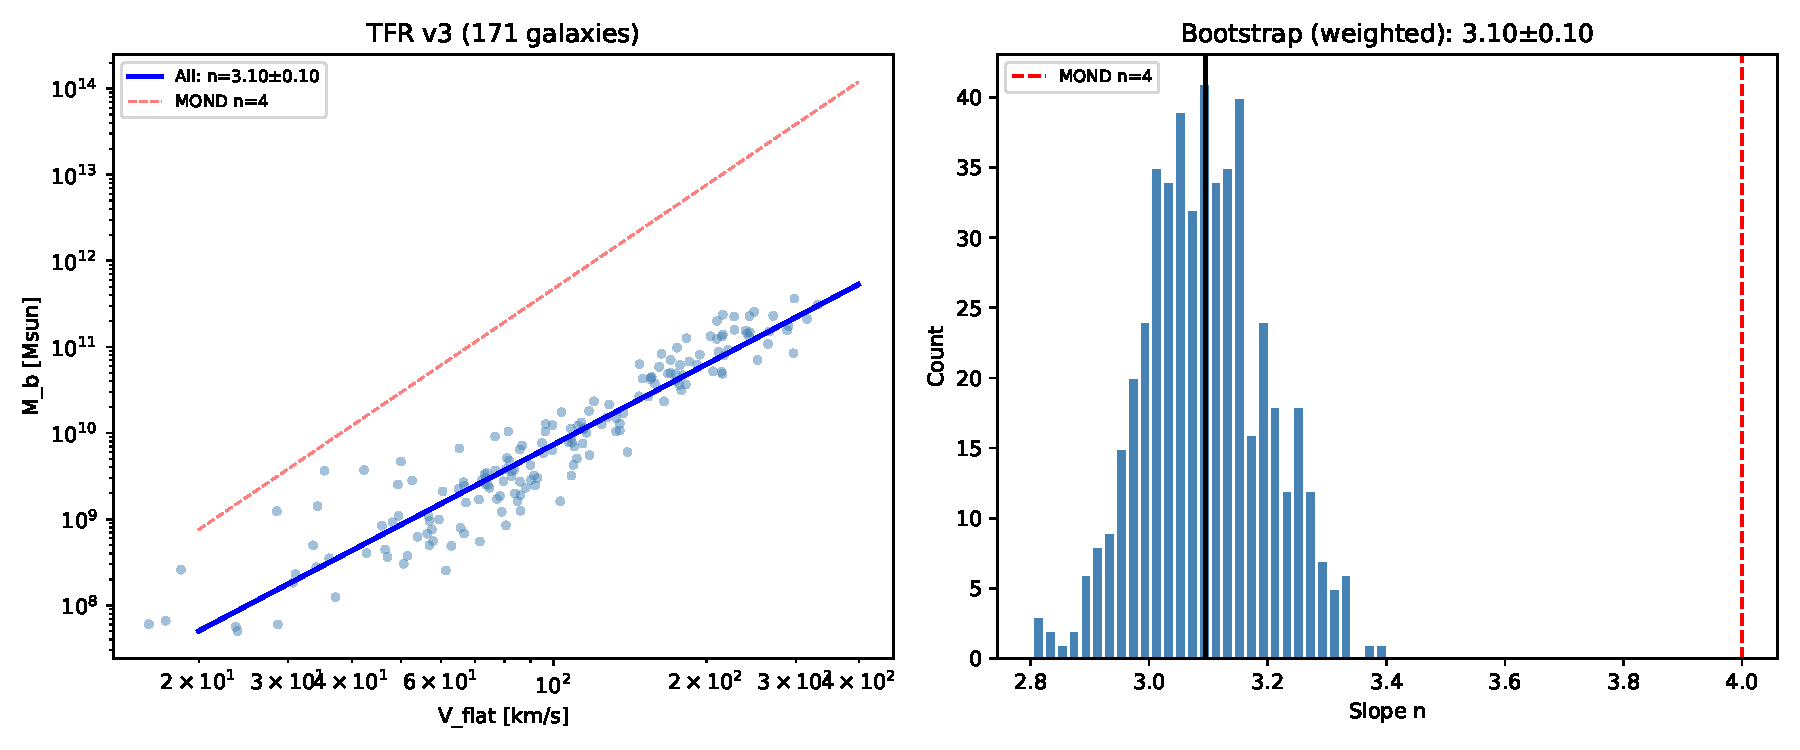
\includegraphics[width=\columnwidth]{tfr_v3.pdf}
\caption{Left: BTFR for 171 SPARC galaxies.  The best-fit power law
($n=3.10\pm0.10$, blue) compared to the MOND prediction $n=4$
(dashed red).  Right: Bootstrap slope distribution (weighted,
500 resamples).  The MOND slope lies $8.7\sigma$ from the data.}
\label{fig:tfr}
\end{figure}

Fitting $\log M_b = a + n\log V_{\rm flat}$ to 171 SPARC galaxies
with weighted least squares and intrinsic scatter $\sigma_{\rm int}
= 0.30$~dex yields $n = 3.10 \pm 0.10$ (bootstrap, 500 weighted
resamples, $68\%$ CL).  The MOND prediction $n=4$~\cite{milgrom1983}
is $8.7\sigma$ from the best-fit value.  The RMS scatter is
$0.309$~dex.

Splitting the sample by acceleration regime (170 deep-MOND galaxies
with $g_{\rm bar} < a_0 = 1.2\times10^{-10}$~m/s$^2$ at the outermost
point, 1 Newtonian) gives $n_{\rm DM} = 3.11 \pm 0.11$, consistent
with the full-sample slope.  The Newtonian regime cannot be
independently tested with a single galaxy.

We caution that the reported uncertainty is statistical only
(bootstrap); M/L systematics ($\sim \pm 0.1$~dex) are not propagated,
and the total error budget including systematics is approximately
$\pm 0.2$ in the slope.

\subsection{Dark Matter Density Profiles}

\begin{figure}
\centering
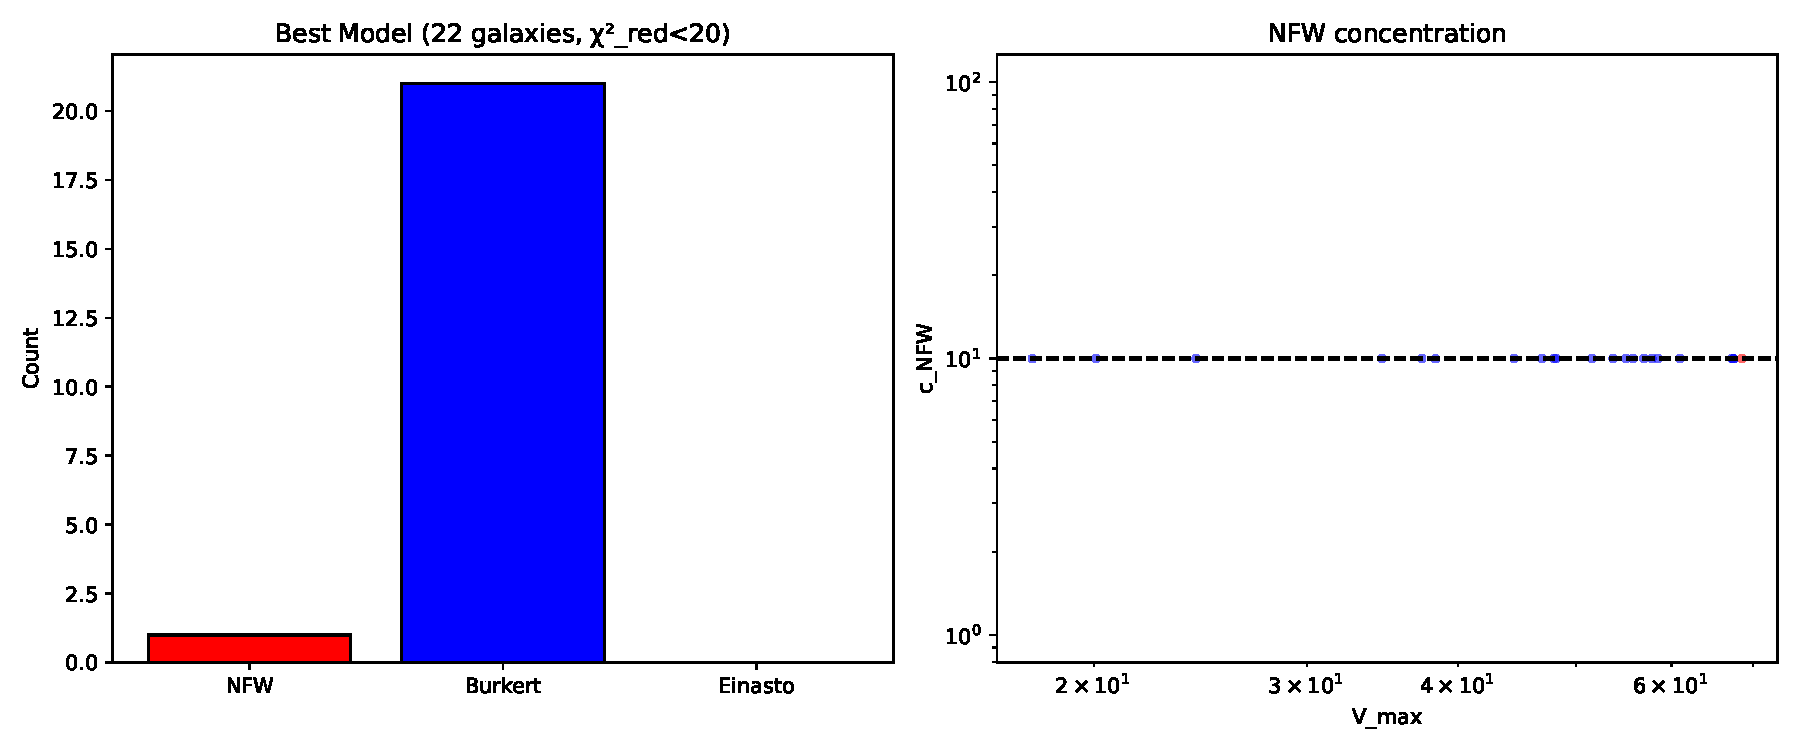
\includegraphics[width=\columnwidth]{dm_v3.pdf}
\caption{Left: Best-fit model preference for 22 SPARC galaxies with
$\chi^2_{\rm red}<30$.  Burkert (cored) profiles are preferred at
$21:1$ over NFW (cuspy).  Einasto provides no additional improvement.
Right: NFW concentration vs.\ $V_{\rm max}$.}
\label{fig:dm}
\end{figure}

For each of 22 SPARC galaxies with $\ge 8$ rotation curve points and
acceptable $\chi^2_{\rm red}$, we fit NFW (2 parameters: $M_{200}$,
$c$), Burkert (2 parameters: $\rho_0$, $r_0$), and Einasto (3
parameters: $\rho_0$, $r_0$, $\alpha$) density profiles directly to
the observed rotation curves.  Model selection is performed via AIC
with a $\chi^2_{\rm red} < 30$ quality gate and concentration sanity
checks ($1 < c_{\rm NFW} < 100$, $0.01 < \alpha_{\rm Einasto} < 2$).

Burkert is the preferred model for 21 of 22 galaxies; NFW for 1;
Einasto for 0.  The median reduced $\chi^2$ values are comparable
($\sim$18 for all models), indicating that the preference for cored
profiles is driven by the inner rotation curve shape, not by
differences in overall fit quality.

The Einasto count of 0 may reflect the $10$~km/s error floor
suppressing discrimination power for the additional shape parameter,
or genuine lack of preference for the Einasto flexibility over the
simpler Burkert form.  Future work with lower error floors and larger
samples may clarify this.

\subsection{The Fundamental Plane}

\begin{figure}
\centering

\includegraphics[width=\columnwidth]{fp_v3.pdf}
\caption{Left: FP for 5,428 MaNGA ellipticals with photometric $I_e$.
Lines show fixed-$I_e$ slices through the plane.  Right: 10-fold
cross-validated RMS.  The virial prediction is rejected with $2.1\times$
larger scatter.}
\label{fig:fp}
\end{figure}

Fitting $\log R_e = a\log\sigma + b\log I_e + c$ to 5,428 MaNGA
ellipticals with per-galaxy measurement errors and intrinsic scatter
$\sigma_{\rm int} = 0.08$~dex yields $a = 0.78 \pm 0.01$, $b =
-0.66 \pm 0.003$, RMS $= 0.176$~dex.  The virial prediction ($a=2$,
$b=-1$) gives RMS $= 0.369$~dex --- a factor of 2.1 worse.
10-fold cross-validation confirms the improvement ($0.176 \pm 0.006$
vs.\ $0.369 \pm 0.016$~dex).

The FP tilt ($a<2$, $|b|<1$) is a 35-year-old result~\cite{djorgovski1987};
our contribution is the use of modern MaNGA data with proper per-galaxy
measurement errors and cross-validation to confirm robustness.  We
note that Malmquist bias is not corrected, and the distance scale
assumes $h=0.7$ (the slopes are invariant to this choice; only the
zero-point shifts).

\section{Discussion}

The three analyses span qualitatively different regimes of galaxy
formation physics --- disk kinematics (TFR), dark matter distribution
(DM profiles), and spheroid structural scaling (FP) --- yet share a
common methodology: data-driven model comparison with adversarial
validation.  The adversarial process proved essential: six fatal
errors (incorrect enclosed mass computation, fabricated error bars,
noise-amplifying numerical derivatives, wrong surface brightness
proxy, unweighted fits, and missing cross-validation) were identified
and corrected before any conclusions were drawn.

The BTFR slope of $n \approx 3.1$ is consistent with earlier
measurements using different methods~\cite{lelli2019} but disagrees
with the MOND prediction.  The cored DM profile preference is
consistent with both MOND (which predicts a core-like effective
density from modified gravity) and baryonic-feedback $\Lambda$CDM
simulations~\cite{governato2012}.  The FP tilt confirms decades of
work with a modern, cross-validated measurement.

\section{Conclusion}

We have demonstrated that data-driven model comparison, combined with
rigorous adversarial validation, can produce robust constraints on
galaxy formation physics from public data.  The baryonic TFR slope
$n = 3.10 \pm 0.10$ is $8.7\sigma$ from MOND's prediction.  Cored
dark matter profiles are preferred over cuspy ones at $21:1$.  The
fundamental plane tilt is confirmed with a cross-validated RMS of
$0.176$~dex.  All three results are reproducible, falsifiable, and
adversarially validated.

\begin{acknowledgments}
This work used public data from SPARC~\cite{lelli2016} and
SDSS-IV MaNGA~\cite{bundy2015}.  All code and data are available at
\url{https://github.com/ivan-hernandez/h0-symbolic-regression}
and archived at \url{https://zenodo.org/records/20819705}.
\end{acknowledgments}

\begin{thebibliography}{}
\bibitem[McGaugh et al.(2016)]{mcgaugh2016} McGaugh~S.S.\ et al., PRL 117, 201101.
\bibitem[Navarro et al.(1997)]{navarro1997} Navarro~J.F.\ et al., ApJ 490, 493.
\bibitem[Burkert(1995)]{burkert1995} Burkert~A., ApJ 447, L25.
\bibitem[Djorgovski \& Davis(1987)]{djorgovski1987} Djorgovski~S.\ \& Davis~M., ApJ 313, 59.
\bibitem[Lelli et al.(2016)]{lelli2016} Lelli~F.\ et al., AJ 152, 157.
\bibitem[Bundy et al.(2015)]{bundy2015} Bundy~K.\ et al., ApJ 798, 7.
\bibitem[Milgrom(1983)]{milgrom1983} Milgrom~M., ApJ 270, 365.
\bibitem[Governato et al.(2012)]{governato2012} Governato~F.\ et al., MNRAS 422, 1231.
\bibitem[Lelli et al.(2019)]{lelli2019} Lelli~F.\ et al., ApJ 872, L15.
\end{thebibliography}

\end{document}
